

\section{Anhang}

%\appendix
\subsection{Code-Dokumentation der Python-Bibliothek util}

Im folgenden Anhang ist die Dokumentation der Python-Bibliothek enthalten. Jede Funktion wird mit einer kurzen Beschreibung sowie dem zugehörigen Code vorgestellt.
Die Dokumentation der Library util.py ist ebenfalls als HTML-Datei \texttt{util.html} dieser Arbeit beigefügt.










\subsubsection*{\colorbox{lightgray}{\texttt{\textbf{\color{green} def} \color{blue} apply\_rot\_matrix}\textbf{\texttt{(mesh, rot\_mat):}}}}
Wendet eine Rotationsmatrix auf ein Mesh-Objekt an, indem die Matrix in ein Quaternion umgewandelt wird und auf das bestehende Quaternion des Meshs angewendet wird.

% Parameter Abschnitt
\noindent \textbf{Parameter:} \vspace{-6ex} \\
\begin{itemize}
    \setlength{\itemindent}{1em}
    \item \texttt{mesh}: Das Mesh-Objekt, auf das die Rotation angewendet werden soll. Erwartet wird, dass das Mesh ein quaternion-Attribut besitzt.
    \item \texttt{rot\_mat}: Die Rotationsmatrix, die auf das Mesh angewendet werden soll. Muss eine 3x3 Matrix sein.
\end{itemize}

% Rückgabewert Abschnitt
\noindent \textbf{Rückgabewert:} \vspace{-6ex} \\
\begin{itemize}
    \setlength{\itemindent}{1em}
    \item Keine Rückgabe, das Mesh-Objekt wird direkt modifiziert.
\end{itemize}

--------------------------------------------------------------------------------------

\label{sec:apply_rot_matrix_animated}
\subsubsection*{
  \colorbox{lightgray}{
    \begin{minipage}{\textwidth}
      \texttt{\textbf{\color{green} def} \color{blue} apply\_rot\_matrix\_animated} \\
      \texttt{\textbf{(mesh, rot\_mat, speed=100, show\_rot\_axis=True):}}
    \end{minipage}
  }
}
%\subsubsection*{\colorbox{lightgray}{\texttt{\textbf{\color{green} def} \color{blue} apply\_rot\_matrix\_animated}\textbf{\texttt{(mesh, rot\_mat, speed=100, show\_rot\_axis=True):}}}}
Wendet eine Rotationsmatrix auf ein Mesh an und rotiert es animiert mit einer gegebenen Geschwindigkeit. Dabei kann optional eine Rotationsachse angezeigt werden.

% Parameter Abschnitt
\noindent \textbf{Parameter:} \vspace{-6ex} \\
\begin{itemize}
    \setlength{\itemindent}{1em}
    \item \texttt{mesh}: Das Mesh, das rotiert werden soll.
    \item \texttt{rot\_mat}: Die Rotationsmatrix, die auf das Mesh angewendet werden soll.
    \item \texttt{speed}: Die Geschwindigkeit der Animation, angegeben als Anzahl der Frames pro Sekunde. Standardwert ist \texttt{100}.
    \item \texttt{show\_rot\_axis}: Ein Boolean-Wert, der angibt, ob die Rotationsachse angezeigt werden soll. Standardwert ist \texttt{True}.
\end{itemize}

% Rückgabewert Abschnitt
\noindent \textbf{Rückgabewert:} \vspace{-6ex} \\
\begin{itemize}
    \setlength{\itemindent}{1em}
    \item Keine Rückgabe (Void-Funktion).
\end{itemize}

--------------------------------------------------------------------------------------


\subsubsection*{\colorbox{lightgray}{\texttt{\textbf{\color{green} def} \color{blue} compute\_normals}\textbf{\texttt{(vertices, indices):}}}}
Generiert die Normalen für alle Dreiecke, die sich aus \texttt{vertices} und \texttt{indices} ergeben.

% Parameter Abschnitt
\noindent \textbf{Parameter:} \vspace{-6ex} \\
\begin{itemize}
    \setlength{\itemindent}{1em}
    \item \texttt{vertices}: Die Punkte im Raum, aus denen die Dreiecke bestehen, für die die Normalen berechnet werden, als Array.
    \item \texttt{indices}: Die Indizes zum Verbinden der Punkte zu Dreiecken, für welche dann die Normalen berechnet werden, als Array.
\end{itemize}

% Rückgabewert Abschnitt
\noindent \textbf{Rückgabewert:} \vspace{-6ex} \\
\begin{itemize}
    \setlength{\itemindent}{1em}
    \item Ein Array, welches die Normalen enthält.
\end{itemize}

--------------------------------------------------------------------------------------


\subsubsection*{\colorbox{lightgray}{\texttt{\textbf{\color{green} def} \color{blue} create\_axes}\textbf{\texttt{(len, font\_scale=0.4, show\_labels=True, name=''):}}}}
Erstellt ein 3D-Koordinatensystem mit den Achsen X, Y, Z und optionalen Beschriftungen.

% Parameter Abschnitt
\noindent \textbf{Parameter:} \vspace{-6ex} \\
\begin{itemize}
    \setlength{\itemindent}{1em}
    \item \texttt{len}: Länge der Achsen.
    \item \texttt{font\_scale}: Skalierung der Schriftgröße für die Achsenbeschriftungen.
    \item \texttt{show\_labels}: Boolescher Wert, der angibt, ob die Achsenbeschriftungen angezeigt werden sollen.
    \item \texttt{name}: Optionaler Name, der in der Mitte des Koordinatensystems angezeigt wird.
\end{itemize}

% Rückgabewert Abschnitt
\noindent \textbf{Rückgabewert:} \vspace{-6ex} \\
\begin{itemize}
    \setlength{\itemindent}{1em}
    \item Ein 3D-Objekt (Group), das das Koordinatensystem mit Achsen und optionalen Beschriftungen enthält.
\end{itemize}

--------------------------------------------------------------------------------------



\subsubsection*{
  \colorbox{lightgray}{
    \begin{minipage}{\textwidth}
      \texttt{\textbf{\color{green} def} \color{blue} create\_cylinder} \\
      \texttt{\textbf{(pos, radiusTop=1, radiusBottom=1, height=2, radialSegments=32, color=[255, 0, 0], transparent=True):}}
    \end{minipage}
  }
}
%\subsubsection*{\colorbox{lightgray}{\texttt{\textbf{\color{green} def} \color{blue} create\_cylinder}\textbf{\texttt{(pos, radiusTop=1, radiusBottom=1, height=2, radialSegments=32, color=[255, 0, 0], transparent=True):}}}}
Erstellt ein Zylinder-Mesh mit der angegebenen Position, Größe und Farbe.

% Parameter Abschnitt
\noindent \textbf{Parameter:} \vspace{-6ex} \\
\begin{itemize}
    \setlength{\itemindent}{1em}
    \item \texttt{pos}: Die Position des Zylinders als Array oder Tuple \texttt{[x, y, z]}.
    \item \texttt{radiusTop}: Der Radius des Zylinders an der Oberseite. Standardwert ist \texttt{1}.
    \item \texttt{radiusBottom}: Der Radius des Zylinders an der Unterseite. Standardwert ist \texttt{1}.
    \item \texttt{height}: Die Höhe des Zylinders. Standardwert ist \texttt{2}.
    \item \texttt{radialSegments}: Die Anzahl der radialen Segmente des Zylinders, die die Auflösung rund um den Zylinder bestimmen. Standardwert ist \texttt{32}.
    \item \texttt{color}: Die Farbe des Zylinders als Array \texttt{[R, G, B]}, wobei jede Komponente im Bereich 0-255 liegt. Standardwert ist \texttt{[255, 0, 0]} (Rot).
    \item \texttt{transparent}: Ein Boolean-Wert, der angibt, ob das Material transparent sein soll. Standardmäßig \texttt{True}.
\end{itemize}

% Rückgabewert Abschnitt
\noindent \textbf{Rückgabewert:} \vspace{-6ex} \\
\begin{itemize}
    \setlength{\itemindent}{1em}
    \item Ein Mesh-Objekt, das den Zylinder darstellt, mit der angegebenen Position, Größe und Farbe.
\end{itemize}

--------------------------------------------------------------------------------------


\subsubsection*{
  \colorbox{lightgray}{
    \begin{minipage}{\textwidth}
      \texttt{\textbf{\color{green} def} \color{blue} create\_box}\textbf{\textbf{\texttt{(pos, width, height, depth, color=[0, 255, 0], transparent=True):}}}
    \end{minipage}
  }
}
Erzeugt ein Quader-Mesh (Box) mit der angegebenen Position, Größe und Farbe.

% Parameter Abschnitt
\noindent \textbf{Parameter:} \vspace{-6ex} \\
\begin{itemize}
    \setlength{\itemindent}{1em}
    \item \texttt{pos}: Die Position des Quaders als Array oder Tuple \texttt{[x, y, z]}.
    \item \texttt{width}: Die Breite des Quaders.
    \item \texttt{height}: Die Höhe des Quaders.
    \item \texttt{depth}: Die Tiefe des Quaders.
    \item \texttt{color}: Die Farbe des Quaders als Array \texttt{[R, G, B]}, wobei jede Komponente im Bereich 0-255 liegt. Standardmäßig grün \texttt{[0, 255, 0]}.
    \item \texttt{transparent}: Ein Boolean-Wert, der angibt, ob das Material transparent sein soll. Standardmäßig \texttt{True}.
\end{itemize}

% Rückgabewert Abschnitt
\noindent \textbf{Rückgabewert:} \vspace{-6ex} \\
\begin{itemize}
    \setlength{\itemindent}{1em}
    \item Ein Mesh-Objekt, das den Quader darstellt, mit der angegebenen Position, Größe und Farbe.
\end{itemize}

--------------------------------------------------------------------------------------

\subsubsection*{\colorbox{lightgray}{\texttt{\textbf{\color{green} def} \color{blue} create\_grid\_XY}\textbf{\texttt{(size, density):}}}}
Erstellt ein 3D-Gitter im XY-Plane mit der angegebenen Größe und Dichte.

% Parameter Abschnitt
\noindent \textbf{Parameter:} \vspace{-6ex} \\
\begin{itemize}
    \setlength{\itemindent}{1em}
    \item \texttt{size}: Die Größe des Gitters (die Ausdehnung in X- und Y-Richtung).
    \item \texttt{density}: Die Dichte des Gitters, die angibt, wie viele Linien innerhalb des Gitters erstellt werden.
\end{itemize}

% Rückgabewert Abschnitt
\noindent \textbf{Rückgabewert:} \vspace{-6ex} \\
\begin{itemize}
    \setlength{\itemindent}{1em}
    \item Ein 3D-Objekt (Group), das das Gitter mit Linien im XY-Plane enthält.
\end{itemize}

--------------------------------------------------------------------------------------

\subsubsection*{\colorbox{lightgray}{\texttt{\textbf{\color{green} def} \color{blue} create\_grid\_XZ}\textbf{\texttt{(size, density):}}}}
Erstellt ein 3D-Gitter im XZ-Plane mit der angegebenen Größe und Dichte.

% Parameter Abschnitt
\noindent \textbf{Parameter:} \vspace{-6ex} \\
\begin{itemize}
    \setlength{\itemindent}{1em}
    \item \texttt{size}: Die Größe des Gitters (die Ausdehnung in X- und Z-Richtung).
    \item \texttt{density}: Die Dichte des Gitters, die angibt, wie viele Linien innerhalb des Gitters erstellt werden.
\end{itemize}

% Rückgabewert Abschnitt
\noindent \textbf{Rückgabewert:} \vspace{-6ex} \\
\begin{itemize}
    \setlength{\itemindent}{1em}
    \item Ein 3D-Objekt (Group), das das Gitter mit Linien im XZ-Plane enthält.
\end{itemize}

--------------------------------------------------------------------------------------

\subsubsection*{\colorbox{lightgray}{\texttt{\textbf{\color{green} def} \color{blue} create\_differential\_robot}\textbf{\texttt{():}}}}
Erzeugt einen zylinderförmigen Roboter mit Differentialantrieb. Der Roboter hat zwei Räder.

% Parameter Abschnitt
\noindent \textbf{Parameter:} \vspace{-6ex} \\
\begin{itemize}
    \setlength{\itemindent}{1em}  % Einrückung für die Punkte
    \item Keine Parameter.
\end{itemize}

% Rückgabewert Abschnitt
\noindent \textbf{Rückgabewert:} \vspace{-6ex} \\
\begin{itemize}
    \setlength{\itemindent}{1em}  % Einrückung für die Punkte
    \item Ein 3D-Objekt (Mesh) das den Differentialroboter darstellt.
\end{itemize}

--------------------------------------------------------------------------------------


\subsubsection*{\colorbox{lightgray}{\texttt{\textbf{\color{green} def} \color{blue} euler\_to\_quaternion}\textbf{\texttt{(angles, order='ZYZ'):}}}}
Wandelt Eulerwinkel in ein Quaternion um.

% Parameter Abschnitt
\noindent \textbf{Parameter:} \vspace{-6ex} \\
\begin{itemize}
    \setlength{\itemindent}{1em}
    \item \texttt{angles}: Die Eulerwinkel in Grad. Diese müssen in der Reihenfolge angegeben werden, wie es \texttt{order} vorgibt, z.\,B.\ \texttt{angles=[y, x, z]}, \texttt{order="YXZ"}.
    \item \texttt{order}: Rotationsreihenfolge für die Eulerwinkel als String.
\end{itemize}

% Rückgabewert Abschnitt
\noindent \textbf{Rückgabewert:} \vspace{-6ex} \\
\begin{itemize}
    \setlength{\itemindent}{1em}
    \item Das Quaternion als Array.
\end{itemize}

--------------------------------------------------------------------------------------


\subsubsection*{\colorbox{lightgray}{\texttt{\textbf{\color{green} def} \color{blue} euler\_to\_rot\_mat}\textbf{\texttt{(angles, order='ZYZ'):}}}}
Wandelt Eulerwinkel in eine Rotationsmatrix um.

% Parameter Abschnitt
\noindent \textbf{Parameter:} \vspace{-6ex} \\
\begin{itemize}
    \setlength{\itemindent}{1em}
    \item \texttt{angles}: Die Eulerwinkel in Grad. Diese müssen in der Reihenfolge angegeben werden, wie es \texttt{order} vorgibt, z.\,B.\ \texttt{angles=[y, x, z]}, \texttt{order="YXZ"}.
    \item \texttt{order}: Rotationsreihenfolge für die Eulerwinkel als String.
\end{itemize}

% Rückgabewert Abschnitt
\noindent \textbf{Rückgabewert:} \vspace{-6ex} \\
\begin{itemize}
    \setlength{\itemindent}{1em}
    \item Die Rotationsmatrix als mehrdimensionales Array.
\end{itemize}

--------------------------------------------------------------------------------------

\label{sec:line_wheel_driven_robot}
\subsubsection*{\colorbox{lightgray}{\texttt{\textbf{\color{green} def} \color{blue} line\_wheel\_driven\_robot}\textbf{\texttt{(dummy, vel, steps):}}}}
Simuliert die Bewegung eines radgetriebenen Roboters entlang einer Linie und erzeugt dabei Liniensegmente zur Visualisierung des Pfades.

Bei jedem Schritt wird das Dummy-Objekt gemäß der gegebenen Geschwindigkeit bewegt. In regelmäßigen Abständen (alle 64 Schritte) wird ein Liniensegment vom Startpunkt dieses Abschnitts zum aktuellen Punkt erstellt, um die Trajektorie sichtbar zu machen.

% Parameter Abschnitt
\noindent \textbf{Parameter:} \vspace{-6ex} \\
\begin{itemize}
    \setlength{\itemindent}{1em}
    \item \texttt{dummy}: Ein Mesh-Objekt, das die Position und Orientierung des Roboters repräsentiert.
    \item \texttt{vel}: Ein Geschwindigkeitsvektor \([v_x, v_y, \omega_z]\), bestehend aus Translation in lokaler X/Y-Richtung und Rotation um Z.
    \item \texttt{steps}: Anzahl der Bewegungs-Iterationen (Zeitschritte).
\end{itemize}

% Rückgabewert Abschnitt
\noindent \textbf{Rückgabewert:} \vspace{-6ex} \\
\begin{itemize}
    \setlength{\itemindent}{1em}
    \item Eine \texttt{three.Group}, die alle erzeugten Liniensegmente enthält (als Trajektorie).
\end{itemize}

--------------------------------------------------------------------------------------


\subsubsection*{\colorbox{lightgray}{\texttt{\textbf{\color{green} def} \color{blue} move}\textbf{\texttt{(robot, vel, steps=1):}}}}
Bewegt ein Roboterobjekt in mehreren Schritten entsprechend der gegebenen Geschwindigkeit und Rotation.

Die Funktion kombiniert Translation und Rotation:

Zuerst wird eine Rotation um die Z-Achse angewendet, basierend auf dem dritten Element des Geschwindigkeitsvektors \texttt{vel[2]}.
Anschließend wird eine Translation basierend auf der aktuellen Ausrichtung (Z-Rotation) des Roboters ausgeführt.
Die Bewegung wird für eine angegebene Anzahl von Schritten (\texttt{steps}) wiederholt.
Nach jeweils 4 Schritten erfolgt eine kurze Pause zur visuellen Glättung.

% Parameter Abschnitt
\noindent \textbf{Parameter:} \vspace{-6ex} \\
\begin{itemize}
    \setlength{\itemindent}{1em}
    \item \texttt{robot}: Das Objekt (z.B. ein Mesh), das bewegt werden soll. Es muss \texttt{quaternion} und \texttt{position} Attribute besitzen.
    \item \texttt{vel}: Ein Geschwindigkeitsvektor \texttt{[v\_x, v\_y, $\omega$\_z]}, wobei \texttt{v\_x} und \texttt{v\_y} die Translation in der lokalen X- und Y-Richtung und \texttt{$\omega$\_z} die Rotation um die Z-Achse ist (in Radiant).
    \item \texttt{steps}: Die Anzahl der Schritte, die die Bewegung ausführen soll (Standard: 1).
\end{itemize}

% Rückgabewert Abschnitt
\noindent \textbf{Rückgabewert:} \vspace{-6ex} \\
\begin{itemize}
    \setlength{\itemindent}{1em}
    \item Die finale Position des Roboters nach der Bewegung.
\end{itemize}

--------------------------------------------------------------------------------------


\subsubsection*{\colorbox{lightgray}{\texttt{\textbf{\color{green} def} \color{blue} order\_angles}\textbf{\texttt{(x, y, z, order):}}}}
Ordnet die übergebenen Eulerwinkel nach \texttt{order} und gibt diese als Array zurück.

% Parameter Abschnitt
\noindent \textbf{Parameter:} \vspace{-6ex} \\
\begin{itemize}
    \setlength{\itemindent}{1em}
    \item \texttt{x}: Eulerwinkel um \texttt{x}.
    \item \texttt{y}: Eulerwinkel um \texttt{y}.
    \item \texttt{z}: Eulerwinkel um \texttt{z}.
    \item \texttt{order}: Die Reihenfolge, in der die Eulerwinkel geordnet werden sollen.
\end{itemize}

% Rückgabewert Abschnitt
\noindent \textbf{Rückgabewert:} \vspace{-6ex} \\
\begin{itemize}
    \setlength{\itemindent}{1em}
    \item Die geordneten Eulerwinkel als Array.
\end{itemize}

--------------------------------------------------------------------------------------


\subsubsection*{\colorbox{lightgray}{\texttt{\textbf{\color{green} def} \color{blue} quaternion\_multiply}\textbf{\texttt{(q1, q2):}}}}
Multipliziert zwei Quaternions.

% Parameter Abschnitt
\noindent \textbf{Parameter:} \vspace{-6ex} \\
\begin{itemize}
    \setlength{\itemindent}{1em}
    \item \texttt{q1}: Das erste Quaternion als Liste oder Array \([x, y, z, w]\).
    \item \texttt{q2}: Das zweite Quaternion als Liste oder Array \([x, y, z, w]\).
\end{itemize}

% Rückgabewert Abschnitt
\noindent \textbf{Rückgabewert:} \vspace{-6ex} \\
\begin{itemize}
    \setlength{\itemindent}{1em}
    \item Das Ergebnis der Quaternion-Multiplikation als Liste \([x, y, z, w]\).
\end{itemize}

--------------------------------------------------------------------------------------



\subsubsection*{\colorbox{lightgray}{\texttt{\textbf{\color{green} def} \color{blue} quaternion\_to\_euler}\textbf{\texttt{(x, y, z, w, order='ZYZ'):}}}}
Wandelt ein Quaternion in Eulerwinkel um. Dabei wird die übergebene Rotationsreihenfolge für die Eulerwinkel beachtet.

% Parameter Abschnitt
\noindent \textbf{Parameter:} \vspace{-6ex} \\
\begin{itemize}
    \setlength{\itemindent}{1em}
    \item \texttt{x}: x-Komponente des Quaternions.
    \item \texttt{y}: y-Komponente des Quaternions.
    \item \texttt{z}: z-Komponente des Quaternions.
    \item \texttt{w}: w-Komponente des Quaternions.
    \item \texttt{order}: Rotationsreihenfolge für die Eulerwinkel als String.
\end{itemize}

% Rückgabewert Abschnitt
\noindent \textbf{Rückgabewert:} \vspace{-6ex} \\
\begin{itemize}
    \setlength{\itemindent}{1em}
    \item Die Eulerwinkel als Array in der Reihenfolge, wie es \texttt{order} vorgibt, z.\,B. bei \texttt{order="ZXY"}: $[z, x, y]$.
\end{itemize}

--------------------------------------------------------------------------------------


\subsubsection*{\colorbox{lightgray}{\texttt{\textbf{\color{green} def} \color{blue} rot\_axis\_from\_rot\_mat}\textbf{\texttt{(rot\_mat):}}}}
Gibt die Rotationsachse von rot\_mat zurück.

% Parameter Abschnitt
\noindent \textbf{Parameter:} \vspace{-6ex} \\
\begin{itemize}
    \setlength{\itemindent}{1em}  % Einrückung für die Punkte
    \item \texttt{rot\_mat}: Die Rotationsmatrix als mehrdimensionales Array.
\end{itemize}

% Rückgabewert Abschnitt
\noindent \textbf{Rückgabewert:} \vspace{-6ex} \\
\begin{itemize}
    \setlength{\itemindent}{1em}  % Einrückung für die Punkte
    \item Rotationsachse als normalisierter Vektor z.B [x,y,z].
\end{itemize}

--------------------------------------------------------------------------------------



\subsubsection*{\colorbox{lightgray}{\texttt{\textbf{\color{green} def} \color{blue} rot\_matrix\_to\_euler}\textbf{\texttt{(rot\_mat, order='ZYZ'):}}}}
Wandelt eine Rotationsmatrix in Eulerwinkel um.

% Parameter Abschnitt
\noindent \textbf{Parameter:} \vspace{-6ex} \\
\begin{itemize}
    \setlength{\itemindent}{1em}
    \item \texttt{rot\_mat}: Die Rotationsmatrix.
    \item \texttt{order}: Rotationsreihenfolge für die Eulerwinkel als String.
\end{itemize}

% Rückgabewert Abschnitt
\noindent \textbf{Rückgabewert:} \vspace{-6ex} \\
\begin{itemize}
    \setlength{\itemindent}{1em}
    \item Die Eulerwinkel. Diese werden in der Reihenfolge zurückgegeben, wie es \texttt{order} vorgibt, z.\,B.\ \texttt{order="ZXY"} $\rightarrow$ $[Z, X, Y]$.
\end{itemize}

--------------------------------------------------------------------------------------



\subsubsection*{\colorbox{lightgray}{\texttt{\textbf{\color{green} def} \color{blue} rot\_matrix\_to\_quaternion}\textbf{\texttt{(rot\_mat):}}}}
Wandelt eine Rotationsmatrix in ein Quaternion um.

% Parameter Abschnitt
\noindent \textbf{Parameter:} \vspace{-6ex} \\
\begin{itemize}
    \setlength{\itemindent}{1em}
    \item \texttt{rot\_mat}: Die Rotationsmatrix als mehrdimensionales Array.
\end{itemize}

% Rückgabewert Abschnitt
\noindent \textbf{Rückgabewert:} \vspace{-6ex} \\
\begin{itemize}
    \setlength{\itemindent}{1em}
    \item Das Quaternion als Array.
\end{itemize}

--------------------------------------------------------------------------------------


\subsubsection*{\colorbox{lightgray}{\texttt{\textbf{\color{green} def} \color{blue} rotate}\textbf{\texttt{(mesh, angles, order='ZYZ'):}}}}
Führt eine Rotation eines Mesh-Objekts basierend auf den übergebenen Eulerwinkeln und einer Rotationsreihenfolge durch.

% Parameter Abschnitt
\noindent \textbf{Parameter:} \vspace{-6ex} \\
\begin{itemize}
    \setlength{\itemindent}{1em}
    \item \texttt{mesh}: Das Mesh-Objekt, das rotiert werden soll.
    \item \texttt{angles}: Die Eulerwinkel in Grad, die die Rotation definieren. Die Reihenfolge muss dem angegebenen \texttt{order}-Parameter entsprechen.
    \item \texttt{order}: Die Rotationsreihenfolge als String (z.B. \texttt{"ZYZ"}, \texttt{"XYZ"}, etc.). Standardmäßig \texttt{"ZYZ"}.
\end{itemize}

% Rückgabewert Abschnitt
\noindent \textbf{Rückgabewert:} \vspace{-6ex} \\
\begin{itemize}
    \setlength{\itemindent}{1em}
    \item Es wird keine Rückgabe gemacht, da die Rotation direkt auf das \texttt{mesh}-Objekt angewendet wird.
\end{itemize}

--------------------------------------------------------------------------------------


\label{sec:rotate_animated}
\subsubsection*{\colorbox{lightgray}{\texttt{\textbf{\color{green} def} \color{blue} rotate\_animated}\textbf{\texttt{(mesh, angles, order='ZYZ'):}}}}
Führt eine animierte lokale Rotation eines Mesh-Objekts durch. Die Rotation erfolgt achsweise entsprechend der angegebenen Reihenfolge.

Beispiel: order="YXZ" → angles=[Winkel um Y, Winkel um X, Winkel um Z]

Während der Animation wird die Rotation in drei Schritten durchgeführt – einer pro Achse – und am Ende exakt auf das Ziel-Quaternion gesetzt, um numerische Fehler auszugleichen.

% Parameter Abschnitt
\noindent \textbf{Parameter:} \vspace{-6ex} \\
\begin{itemize}
    \setlength{\itemindent}{1em}
    \item \texttt{mesh}: Das 3D-Mesh-Objekt, das rotiert werden soll.
    \item \texttt{angles}: Eine Liste mit Rotationswinkeln (in Grad), die in der Reihenfolge \texttt{order} angegeben sind.
    \item \texttt{order}: Die Rotationsreihenfolge (z.B. "ZYZ", "YXZ", etc.).
\end{itemize}

% Rückgabewert Abschnitt
\noindent \textbf{Rückgabewert:} \vspace{-6ex} \\
\begin{itemize}
    \setlength{\itemindent}{1em}
    \item Keine Rückgabe (void).
\end{itemize}

--------------------------------------------------------------------------------------



\subsubsection*{\colorbox{lightgray}{\texttt{\textbf{\color{green} def} \color{blue} rotate\_global}\textbf{\texttt{(mesh, angles, order='ZYZ'):}}}}
Führt eine globale Rotation eines Mesh-Objekts durch, basierend auf den übergebenen Eulerwinkeln und einer Rotationsreihenfolge.

% Parameter Abschnitt
\noindent \textbf{Parameter:} \vspace{-6ex} \\
\begin{itemize}
    \setlength{\itemindent}{1em}
    \item \texttt{mesh}: Das Mesh-Objekt, das rotiert werden soll.
    \item \texttt{angles}: Die Eulerwinkel in Grad, die die Rotation definieren. Die Reihenfolge muss dem angegebenen \texttt{order}-Parameter entsprechen.
    \item \texttt{order}: Die Rotationsreihenfolge als String (z.B. \texttt{"ZYZ"}, \texttt{"XYZ"}, etc.). Standardmäßig \texttt{"ZYZ"}.
\end{itemize}

% Rückgabewert Abschnitt
\noindent \textbf{Rückgabewert:} \vspace{-6ex} \\
\begin{itemize}
    \setlength{\itemindent}{1em}
    \item Es wird keine Rückgabe gemacht, da die Rotation direkt auf das \texttt{mesh}-Objekt angewendet wird.
\end{itemize}

--------------------------------------------------------------------------------------


\label{sec:rotate_global_animated}
\subsubsection*{\colorbox{lightgray}{\texttt{\textbf{\color{green} def} \color{blue} rotate\_global\_animated}\textbf{\texttt{(mesh, angles, order='ZYZ'):}}}}
Führt eine animierte globale Rotation eines Mesh-Objekts durch. Die Drehung erfolgt achsweise gemäß der angegebenen Rotationsreihenfolge (z.B. "ZYZ"). Die Winkel in \texttt{angles} müssen in der Reihenfolge der \texttt{order}-Zeichen angegeben werden.

Beispiel: Bei \texttt{order="YXZ"} → \texttt{angles=[Winkel um Y, Winkel um X, Winkel um Z]}

Die Funktion führt die Rotation in drei separaten animierten Phasen durch – jeweils eine für jede Achse in \texttt{order}.

% Parameter Abschnitt
\noindent \textbf{Parameter:} \vspace{-6ex} \\
\begin{itemize}
    \setlength{\itemindent}{1em}
    \item \texttt{mesh}: Das 3D-Objekt (Mesh), das rotiert werden soll.
    \item \texttt{angles}: Eine Liste von Rotationswinkeln (in Grad), entsprechend der Reihenfolge in \texttt{order}.
    \item \texttt{order}: Die Rotationsreihenfolge als String, z.B. "ZYZ", "YXZ", etc.
\end{itemize}

% Rückgabewert Abschnitt
\noindent \textbf{Rückgabewert:} \vspace{-6ex} \\
\begin{itemize}
    \setlength{\itemindent}{1em}
    \item Keine Rückgabe (void).
\end{itemize}

--------------------------------------------------------------------------------------



\subsubsection*{\colorbox{lightgray}{\texttt{\textbf{\color{green} def} \color{blue} set\_rotation}\textbf{\texttt{(mesh, angles, order='ZYZ'):}}}}
Setzt die Rotation eines Mesh-Objekts auf die übergebenen Eulerwinkel und die Rotationsreihenfolge.

% Parameter Abschnitt
\noindent \textbf{Parameter:} \vspace{-6ex} \\
\begin{itemize}
    \setlength{\itemindent}{1em}
    \item \texttt{mesh}: Das Mesh-Objekt, dessen Rotation gesetzt werden soll.
    \item \texttt{angles}: Die Eulerwinkel in Grad, die die gewünschte Rotation definieren. Die Reihenfolge muss dem angegebenen \texttt{order}-Parameter entsprechen.
    \item \texttt{order}: Die Rotationsreihenfolge als String (z.B. \texttt{"ZYZ"}, \texttt{"XYZ"}, etc.). Standardmäßig \texttt{"ZYZ"}.
\end{itemize}

% Rückgabewert Abschnitt
\noindent \textbf{Rückgabewert:} \vspace{-6ex} \\
\begin{itemize}
    \setlength{\itemindent}{1em}
    \item Es wird keine Rückgabe gemacht, da die Rotation direkt auf das \texttt{mesh}-Objekt angewendet wird.
\end{itemize}

--------------------------------------------------------------------------------------



\subsubsection*{\colorbox{lightgray}{\texttt{\textbf{\color{green} def} \color{blue} set\_rotation\_global}\textbf{\texttt{(mesh, angles, order='ZYZ'):}}}}
Setzt die globale Rotation eines Mesh-Objekts auf die übergebenen Eulerwinkel und die Rotationsreihenfolge.

% Parameter Abschnitt
\noindent \textbf{Parameter:} \vspace{-6ex} \\
\begin{itemize}
    \setlength{\itemindent}{1em}
    \item \texttt{mesh}: Das Mesh-Objekt, dessen globale Rotation gesetzt werden soll.
    \item \texttt{angles}: Die Eulerwinkel in Grad, die die gewünschte Rotation definieren. Die Reihenfolge muss dem angegebenen \texttt{order}-Parameter entsprechen.
    \item \texttt{order}: Die Rotationsreihenfolge als String (z.B. \texttt{"ZYZ"}, \texttt{"XYZ"}, etc.). Standardmäßig \texttt{"ZYZ"}.
\end{itemize}

% Rückgabewert Abschnitt
\noindent \textbf{Rückgabewert:} \vspace{-6ex} \\
\begin{itemize}
    \setlength{\itemindent}{1em}
    \item Es wird keine Rückgabe gemacht, da die Rotation direkt auf das \texttt{mesh}-Objekt angewendet wird.
\end{itemize}

--------------------------------------------------------------------------------------


\subsubsection*{\colorbox{lightgray}{\texttt{\textbf{\color{green} def} \color{blue} set\_scale}\textbf{\texttt{(mesh, scale):}}}}
Setzt die Skalierung eines Mesh-Objekts.

% Parameter Abschnitt
\noindent \textbf{Parameter:} \vspace{-6ex} \\
\begin{itemize}
    \setlength{\itemindent}{1em}
    \item \texttt{mesh}: Das Mesh-Objekt, dessen Skalierung angepasst werden soll.
    \item \texttt{scale}: Ein Array, das den Skalierungsfaktor für jede Achse (x, y, z) angibt, z.B. \([1, 2, 1]\).
\end{itemize}

% Rückgabewert Abschnitt
\noindent \textbf{Rückgabewert:} \vspace{-6ex} \\
\begin{itemize}
    \setlength{\itemindent}{1em}
    \item Keine Rückgabe (void).
\end{itemize}

--------------------------------------------------------------------------------------

\subsubsection*{\colorbox{lightgray}{\texttt{\textbf{\color{green} def} \color{blue} set\_scale\_animated}\textbf{\texttt{(mesh, scale):}}}}
Setzt die Skalierung eines Mesh-Objekts animiert, indem es schrittweise die Größe verändert.

% Parameter Abschnitt
\noindent \textbf{Parameter:} \vspace{-6ex} \\
\begin{itemize}
    \setlength{\itemindent}{1em}
    \item \texttt{mesh}: Das Mesh-Objekt, dessen Skalierung angepasst werden soll.
    \item \texttt{scale}: Ein Array, das die Ziel-Skalierungswerte für jede Achse (x, y, z) angibt, z.B. \([1, 2, 1]\).
\end{itemize}

% Rückgabewert Abschnitt
\noindent \textbf{Rückgabewert:} \vspace{-6ex} \\
\begin{itemize}
    \setlength{\itemindent}{1em}
    \item Keine Rückgabe (void).
\end{itemize}

--------------------------------------------------------------------------------------



\subsubsection*{\colorbox{lightgray}{\texttt{\textbf{\color{green} def} \color{blue} set\_translation}\textbf{\texttt{(mesh, vec):}}}}
Setzt die Position eines Mesh-Objekts auf die angegebenen Koordinaten.

% Parameter Abschnitt
\noindent \textbf{Parameter:} \vspace{-6ex} \\
\begin{itemize}
    \setlength{\itemindent}{1em}
    \item \texttt{mesh}: Das Mesh-Objekt, dessen Position gesetzt werden soll.
    \item \texttt{vec}: Der Ziel-Vektor als Array oder Liste \texttt{[x, y, z]}, der die neue Position des Meshs im Raum angibt.
\end{itemize}

% Rückgabewert Abschnitt
\noindent \textbf{Rückgabewert:} \vspace{-6ex} \\
\begin{itemize}
    \setlength{\itemindent}{1em}
    \item Es wird keine Rückgabe gemacht, da die Position des \texttt{mesh}-Objekts direkt gesetzt wird.
\end{itemize}

--------------------------------------------------------------------------------------

\subsubsection*{\colorbox{lightgray}{\texttt{\textbf{\color{green} def} \color{blue} set\_translation\_animated}\textbf{\texttt{(mesh, vec, speed=50.0):}}}}
Bewegt die Position eines Mesh-Objekts animiert von der aktuellen Position zu einer angegebenen Zielposition.

% Parameter Abschnitt
\noindent \textbf{Parameter:} \vspace{-6ex} \\
\begin{itemize}
    \setlength{\itemindent}{1em}
    \item \texttt{mesh}: Das Mesh-Objekt, dessen Position animiert geändert werden soll.
    \item \texttt{vec}: Der Ziel-Vektor als Array oder Liste \texttt{[x, y, z]}, zu dem die Position des Meshs bewegt werden soll.
    \item \texttt{speed}: Die Geschwindigkeit der Animation. Ein höherer Wert bedeutet eine schnellere Bewegung.
\end{itemize}

% Rückgabewert Abschnitt
\noindent \textbf{Rückgabewert:} \vspace{-6ex} \\
\begin{itemize}
    \setlength{\itemindent}{1em}
    \item Es wird keine Rückgabe gemacht, da die Position des \texttt{mesh}-Objekts animiert geändert wird.
\end{itemize}

--------------------------------------------------------------------------------------





\subsubsection*{\colorbox{lightgray}{\texttt{\textbf{\color{green} def} \color{blue} slerp\_quaternion}\textbf{\texttt{(q1, q2, t):}}}}
Führt eine Spherical Linear Interpolation (SLERP) zwischen zwei Quaternionen durch. Interpoliert die Rotation zwischen \texttt{q1} und \texttt{q2} basierend auf dem Interpolationswert \texttt{t}.

% Parameter Abschnitt
\noindent \textbf{Parameter:} \vspace{-6ex} \\
\begin{itemize}
    \setlength{\itemindent}{1em}
    \item \texttt{q1}: Das erste Quaternion, das die Anfangsrotation beschreibt.
    \item \texttt{q2}: Das zweite Quaternion, das die Endrotation beschreibt.
    \item \texttt{t}: Der Interpolationswert, der zwischen 0 und 1 liegen muss. Ein Wert von 0 entspricht der Rotation von \texttt{q1} und ein Wert von 1 entspricht der Rotation von \texttt{q2}.
\end{itemize}

% Rückgabewert Abschnitt
\noindent \textbf{Rückgabewert:} \vspace{-6ex} \\
\begin{itemize}
    \setlength{\itemindent}{1em}
    \item Das interpolierte Quaternion, das die Rotation zwischen \texttt{q1} und \texttt{q2} bei dem gegebenen Wert von \texttt{t} beschreibt.
\end{itemize}

% Fehlerbehandlung Abschnitt
\noindent \textbf{Fehlerbehandlung:} \vspace{-6ex} \\
\begin{itemize}
    \setlength{\itemindent}{1em}
    \item \texttt{ValueError}: Wenn der Interpolationswert \texttt{t} nicht zwischen 0 und 1 liegt.
\end{itemize}

--------------------------------------------------------------------------------------



\subsubsection*{\colorbox{lightgray}{\texttt{\textbf{\color{green} def} \color{blue} translate}\textbf{\texttt{(mesh, vec):}}}}
Verschiebt ein Mesh-Objekt um einen gegebenen Vektor in den drei Raumachsen.

% Parameter Abschnitt
\noindent \textbf{Parameter:} \vspace{-6ex} \\
\begin{itemize}
    \setlength{\itemindent}{1em}
    \item \texttt{mesh}: Das Mesh-Objekt, das verschoben werden soll.
    \item \texttt{vec}: Der Verschiebungsvektor als Array oder Liste \texttt{[x, y, z]}, der die Verschiebung in den jeweiligen Raumachsen angibt.
\end{itemize}

% Rückgabewert Abschnitt
\noindent \textbf{Rückgabewert:} \vspace{-6ex} \\
\begin{itemize}
    \setlength{\itemindent}{1em}
    \item Es wird keine Rückgabe gemacht, da das \texttt{mesh}-Objekt direkt verschoben wird.
\end{itemize}

--------------------------------------------------------------------------------------


\subsubsection*{\colorbox{lightgray}{\texttt{\textbf{\color{green} def} \color{blue} translate\_animated}\textbf{\texttt{(mesh, vec, speed=50.0):}}}}
Bewegt die Position eines Mesh-Objekts animiert um einen angegebenen Vektor von der aktuellen Position.

% Parameter Abschnitt
\noindent \textbf{Parameter:} \vspace{-6ex} \\
\begin{itemize}
    \setlength{\itemindent}{1em}  % Einrückung für die Punkte
    \item \texttt{mesh}: Das Mesh-Objekt, dessen Position animiert geändert werden soll.
    \item \texttt{vec}: Der Verschiebungs-Vektor als Array oder Liste [dx, dy, dz], um den die Position des Meshs verändert werden soll.
    \item \texttt{speed}: Die Geschwindigkeit der Animation. Ein höherer Wert bedeutet eine schnellere Bewegung.
\end{itemize}

% Rückgabewert Abschnitt
\noindent \textbf{Rückgabewert:} \vspace{-6ex} \\
\begin{itemize}
    \setlength{\itemindent}{1em}  % Einrückung für die Punkte
    \item Keine Rückgabe.
\end{itemize}

--------------------------------------------------------------------------------------


\subsubsection*{\colorbox{lightgray}{\texttt{\textbf{\color{green} class} \color{blue} Environment}\textbf{:}}}
Eine 3D-Umgebung, die eine Szene mit Kamera, Lichtquellen, Achsen, Gittern und Widgets für die Interaktivität erstellt.

Diese Klasse erstellt eine 3D-Umgebung mit einer Vielzahl von Features, darunter eine Kamera, Lichtquellen, Achsen- und Gitterdarstellung sowie Steuerungen zur Anpassung von Objekten in der Szene (z.B. Rotation, Skalierung, Translation).

% Parameter Abschnitt
\noindent \textbf{Parameter:} \vspace{-6ex} \\
\begin{itemize}
    \setlength{\itemindent}{1em}  % Einrückung für die Punkte
    \item \texttt{width}: Die Breite der Ansicht in Pixeln (Standard: 700).
    \item \texttt{height}: Die Höhe der Ansicht in Pixeln (Standard: 500).
    \item \texttt{frame}: Ein 3D-Achsenobjekt, das als Referenzrahmen in der Szene hinzugefügt wird (Standard: \texttt{create\_axes(8, name="B")}).
    \item \texttt{grid}: Ein Gitterobjekt, das in der Szene an\-ge\-zeigt wird (Stan\-dard: \\ \texttt{create\_grid\_XY(14, 0.5)}).
    \item \texttt{up}: Die Richtung der "Oben"-Achse, die die Orientierung der Kamera bestimmt (Standard: \([0, 0, 1]\)).
\end{itemize}

\noindent \textbf{Diese Klasse enthält Methoden, um:} \vspace{-6ex} \\
\begin{itemize}
    \setlength{\itemindent}{1em}
    \item Die Sichtbarkeit von Gitter und Achsen zu steuern.
    \item Interaktive Widgets für Objekte zu erstellen (Translation, Rotation, Skalierung).
    \item Objekte der Szene hinzuzufügen.
    \item Globale oder lokale Transformationen auf Objekte anzuwenden.
\end{itemize}

\noindent \textbf{Weitere Features:} \vspace{-6ex} \\
\begin{itemize}
    \setlength{\itemindent}{1em}
    \item Die Umgebung kann mit einer interaktiven Steuerung für Kamera und Objekte angezeigt werden.
    \item Widgets für die Manipulation von Objekten (Translation, Rotation, Skalierung) können zur Szene hinzugefügt werden.
\end{itemize}

--------------------------------------------------------------------------------------

\begin{quote}



    \subsubsection*{\colorbox{lightgray}{\texttt{\textbf{\color{green} def} \color{blue} add}\textbf{(self, objekts):}}}
    Fügt ein oder mehrere Objekte zur Szene hinzu.
    
    % Parameter Abschnitt
    \noindent \textbf{Parameter:} \vspace{-6ex} \\
    \begin{itemize}
        \setlength{\itemindent}{1em}  % Einrückung für die Punkte
        \item \texttt{objekts}: Ein einzelnes Objekt oder eine Liste von Objekten, die zur Szene hinzugefügt werden.
    \end{itemize}
    
    --------------------------------------------------------------------------------------
    
    \label{sec:add_gizmo_controls}
    \subsubsection*{
      \colorbox{lightgray}{
        \begin{minipage}{\textwidth}
          \texttt{\textbf{\color{green} def} \color{blue} add\_gizmo\_controls} 
          \texttt{\textbf{(self, obj, translation=True,}} \\
          \texttt{\textbf{rotation=True, scale=True):}}
        \end{minipage}
      }
    }
    %\subsubsection*{\colorbox{lightgray}{\texttt{\textbf{\color{green} def} \color{blue} add\_gizmo\_controls}\textbf{(self, obj, translation=True,\\ rotation=True, scale=True):}}}
    Fügt ein Gizmo-Steuerelement zur Manipulation eines Objekts in der Umgebung hinzu (Translation, Rotation, Skalierung).
    
    % Parameter Abschnitt
    \noindent \textbf{Parameter:} \vspace{-6ex} \\
    \begin{itemize}
        \setlength{\itemindent}{1em}  % Einrückung für die Punkte
        \item \texttt{obj}: Das Objekt, das manipuliert werden soll.
        \item \texttt{translation}: Wenn True, werden Schieberegler für die Translation angezeigt.
        \item \texttt{rotation}: Wenn True, werden Schieberegler für die Rotation angezeigt.
        \item \texttt{scale}: Wenn True, werden Schieberegler für die Skalierung angezeigt.
    \end{itemize}
    
    --------------------------------------------------------------------------------------
    
    
    \subsubsection*{\colorbox{lightgray}{\texttt{\textbf{\color{green} def} \color{blue} add\_widget}\textbf{(self, widget):}}}
    Fügt ein Widget zur Umgebung hinzu. Dabei kann es sich auch um ein Bündel von Widgets in einer HBox oder einer VBox handeln.
    
    % Parameter Abschnitt
    \noindent \textbf{Parameter:} \vspace{-6ex} \\
    \begin{itemize}
        \setlength{\itemindent}{1em}  % Einrückung für die Punkte
        \item \texttt{widget}: Das Widget, das der Umgebung hinzugefügt werden soll.
    \end{itemize}
    
    --------------------------------------------------------------------------------------
    


    \subsubsection*{\colorbox{lightgray}{\texttt{\textbf{\color{green} def} \color{blue} set\_frame\_widgets}\textbf{(self, bool):}}}
    Aktiviert oder deaktiviert die Anzeige von Frame-Widgets.

    % Parameter Abschnitt
    \noindent \textbf{Parameter:} \vspace{-6ex} \\
    \begin{itemize}
        \setlength{\itemindent}{1em}  % Einrückung für die Punkte
        \item \texttt{bool}: Wenn True, werden die Widgets angezeigt, andernfalls ausgeblendet.
    \end{itemize}

    --------------------------------------------------------------------------------------



    \subsubsection*{\colorbox{lightgray}{\texttt{\textbf{\color{green} def} \color{blue} toggle\_axes}\textbf{(self, change):}}}
    Schaltet die Sichtbarkeit der Achsen um.

    % Parameter Abschnitt
    \noindent \textbf{Parameter:} \vspace{-6ex} \\
    \begin{itemize}
        \setlength{\itemindent}{1em}  % Einrückung für die Punkte
        \item \texttt{change}: Das Ereignis, das diese Funktion auslöst (wird nicht genutzt).
    \end{itemize}

    --------------------------------------------------------------------------------------



    \subsubsection*{\colorbox{lightgray}{\texttt{\textbf{\color{green} def} \color{blue} toggle\_grid}\textbf{(self, change):}}}
    Schaltet die Sichtbarkeit des Gitters um.

    % Parameter Abschnitt
    \noindent \textbf{Parameter:} \vspace{-6ex} \\
    \begin{itemize}
        \setlength{\itemindent}{1em}  % Einrückung für die Punkte
        \item \texttt{change}: Das Ereignis, das diese Funktion auslöst (wird nicht genutzt).
    \end{itemize}

    --------------------------------------------------------------------------------------










\end{quote}


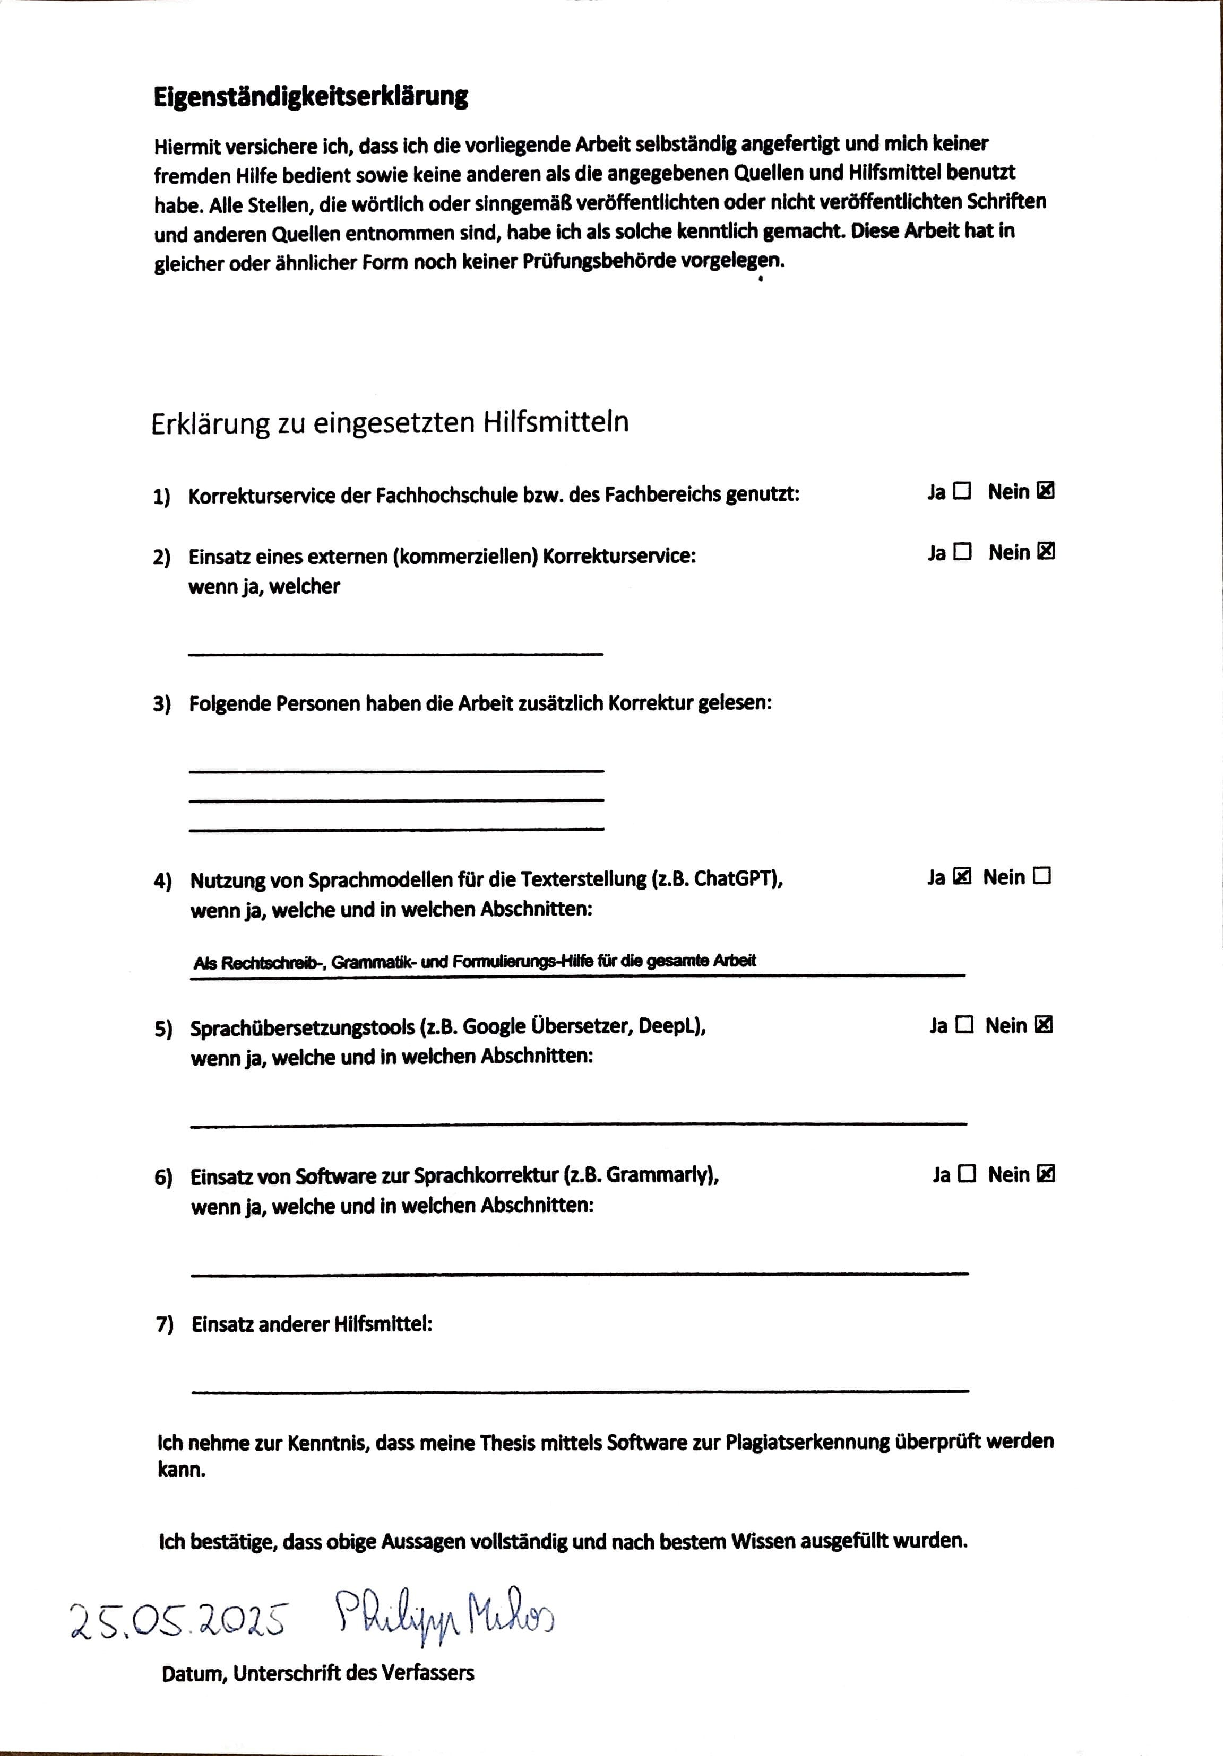
\includepdf[pages=1]{eigenst.pdf}

